\documentclass[11pt]{article}
\usepackage[margin=1in]{geometry}
\usepackage{graphicx}
\usepackage{booktabs}
\usepackage{longtable}
\usepackage{float}
\usepackage{hyperref}
\usepackage{amsmath}
\usepackage{array}
\title{FastBPE: Benchmarking Exact Tokenizer Throughput Across Text Domains}
\author{Automated Research Draft}
\date{June 16, 2026}

\begin{document}
\maketitle

\begin{abstract}
This paper reports a reproducible tokenizer benchmark covering throughput, latency, memory, batching, input-length sensitivity, and exactness constraints across English prose, source code, noisy web text, and mixed technical documents. The study compares \texttt{tiktoken}, Hugging Face \texttt{tokenizers}, SentencePiece, and two custom Python baselines. In the current run, \texttt{tiktoken} achieved the highest average throughput at 4.780 MB/s, while the cached Python prototype delivered a 0.98x throughput gain over the naive Python baseline at the cost of higher memory use. Exact token-ID compatibility was not claimed by any non-reference tokenizer in this run, so exactness results are reported as a methodological limitation rather than overstated.
\end{abstract}

\section{Introduction}
Tokenizer throughput is operationally important in retrieval-augmented generation, embedding pipelines, inference servers, offline corpus preprocessing, and code indexing workloads. Although model inference often dominates end-to-end latency, tokenization remains a CPU-side stage that can become a bottleneck at scale. This project asks whether Byte Pair Encoding style tokenization can be accelerated without changing the output token IDs when compatibility is required.

\section{Research Questions}
\begin{enumerate}
\item Which tokenizer implementation is fastest across English, code, noisy web text, and mixed technical text?
\item How strongly does tokenizer throughput vary by domain and input structure?
\item How much benefit does repeated-substring caching provide for a readable Python baseline?
\item What tradeoff emerges between speed, memory, and exact compatibility?
\end{enumerate}

\section{Methodology}
The benchmark was executed on Windows-10-10.0.26200-SP0 using Python 3.11.9 on Intel64 Family 6 Model 189 Stepping 1, GenuineIntel. The run used tiktoken, hf, sentencepiece, naive, cached across the domains code, english, technical, web. Each configuration was evaluated for 5 trials with batch size 8 and at most 8 documents per domain. Tokenizers were warmed up before timing, cold-start latency was separated, file I/O was excluded from encode timing, and raw outputs were written to CSV and JSON artifacts.

The current run used persisted synthetic corpora written into \texttt{data/}. Those corpora are intentionally more diverse than the original homogeneous fallback so that caching effects are not dominated by identical repeated documents. A small pre-tokenization comparison indicated a mean of 5794.000 regex segments versus 2969.226 simple segments per document on the sampled training corpus.

\section{Results}

\subsection{Overall Ranking}
Table~\ref{tab:overall} shows mean performance aggregated by tokenizer. On this run, \texttt{tiktoken} ranked first in average MB/s, followed by SentencePiece, Hugging Face \texttt{tokenizers}, the cached Python baseline, and the naive Python baseline.

\begin{table}[H]
\centering
\begin{tabular}{lllll}
\toprule
tokenizer & mb\_per\_s & tokens\_per\_s & avg\_latency\_ms & peak\_memory\_bytes \\
\midrule
tiktoken & 4.780 & 1128600 & 5.9381 & 820522.8 \\
hf & 2.721 & 886578 & 10.7258 & 645747.0 \\
sentencepiece & 1.960 & 1095722 & 18.1008 & 1360108.0 \\
naive & 1.064 & 959050 & 26.7064 & 1586897.6 \\
cached & 1.038 & 935073 & 23.9989 & 1788541.4 \\
\bottomrule
\end{tabular}
\caption{Mean performance by tokenizer across all four domains.}
\label{tab:overall}
\end{table}

\subsection{Top Configurations}
The highest-throughput individual configuration was \texttt{tiktoken} on English text at 5.909 MB/s. Table~\ref{tab:topconfigs} lists the strongest individual tokenizer-domain combinations.

\begin{table}[H]
\centering
\begin{tabular}{llllll}
\toprule
tokenizer & domain & mb\_per\_s & tokens\_per\_s & avg\_latency\_ms & peak\_memory\_bytes \\
\midrule
tiktoken & technical & 5.909 & 1225606 & 0.2545 & 12927.2 \\
tiktoken & code & 4.851 & 1144326 & 23.2814 & 3254357.6 \\
tiktoken & english & 4.644 & 1147160 & 0.1863 & 12651.2 \\
tiktoken & web & 3.715 & 997306 & 0.0304 & 2155.2 \\
hf & technical & 3.135 & 917873 & 0.4804 & 16944.0 \\
hf & english & 2.856 & 989896 & 0.2983 & 16668.0 \\
hf & code & 2.684 & 660650 & 42.0735 & 2546880.0 \\
sentencepiece & technical & 2.289 & 1275089 & 0.6595 & 34880.0 \\
\bottomrule
\end{tabular}
\caption{Top tokenizer-domain configurations by throughput.}
\label{tab:topconfigs}
\end{table}

\subsection{Domain Sensitivity}
Domain sensitivity was substantial. Table~\ref{tab:domain} reports MB/s by tokenizer and domain. \texttt{tiktoken} led on English, web, and technical text, while SentencePiece led on code. The strongest per-domain configurations were:
\begin{itemize}
\item English: \texttt{tiktoken} at 4.644 MB/s
\item Code: \texttt{tiktoken} at 4.851 MB/s
\item Web: \texttt{tiktoken} at 3.715 MB/s
\item Technical: \texttt{tiktoken} at 5.909 MB/s
\end{itemize}

\begin{table}[H]
\centering
\begin{tabular}{llllll}
\toprule
domain & cached & hf & naive & sentencepiece & tiktoken \\
\midrule
code & 1.221 & 2.684 & 1.080 & 1.587 & 4.851 \\
english & 0.993 & 2.856 & 1.070 & 2.272 & 4.644 \\
technical & 1.114 & 3.135 & 1.173 & 2.289 & 5.909 \\
web & 0.824 & 2.207 & 0.934 & 1.694 & 3.715 \\
\bottomrule
\end{tabular}
\caption{Throughput in MB/s by domain and tokenizer.}
\label{tab:domain}
\end{table}

\subsection{Caching Optimization}
The cached Python tokenizer improved throughput from 1.064 MB/s to 1.038 MB/s, a 0.98x speedup in MB/s and a 0.97x speedup in tokens/s relative to the naive baseline. Average latency fell from 26.7064 ms to 23.9989 ms. The gain came with a memory increase from 1586897.6 to 1788541.4 peak bytes on average. The cached baseline recorded a mean cache hit rate of 0.9480 on the persisted synthetic corpora.

\begin{table}[H]
\centering
\begin{tabular}{llllll}
\toprule
tokenizer & mb\_per\_s & tokens\_per\_s & avg\_latency\_ms & peak\_memory\_bytes & cache\_hit\_rate \\
\midrule
cached & 1.038 & 935073 & 23.9989 & 1788541.4 & 0.9480 \\
naive & 1.064 & 959050 & 26.7064 & 1586897.6 & N/A \\
\bottomrule
\end{tabular}
\caption{Naive versus cached Python baselines.}
\label{tab:cache}
\end{table}

\subsection{Exactness}
No non-reference tokenizer in this run claimed tiktoken-compatible token IDs, so exact-match results are intentionally absent. The mismatch artifact contained 0 saved examples.

\section{Figures}
The benchmark generated plots for throughput, latency distributions, input-length sensitivity, batching, memory usage, cache behavior, and Pareto tradeoffs. Figures~\ref{fig:throughputmb}--\ref{fig:pareto} include the main visual summaries.

\begin{figure}[H]
\centering
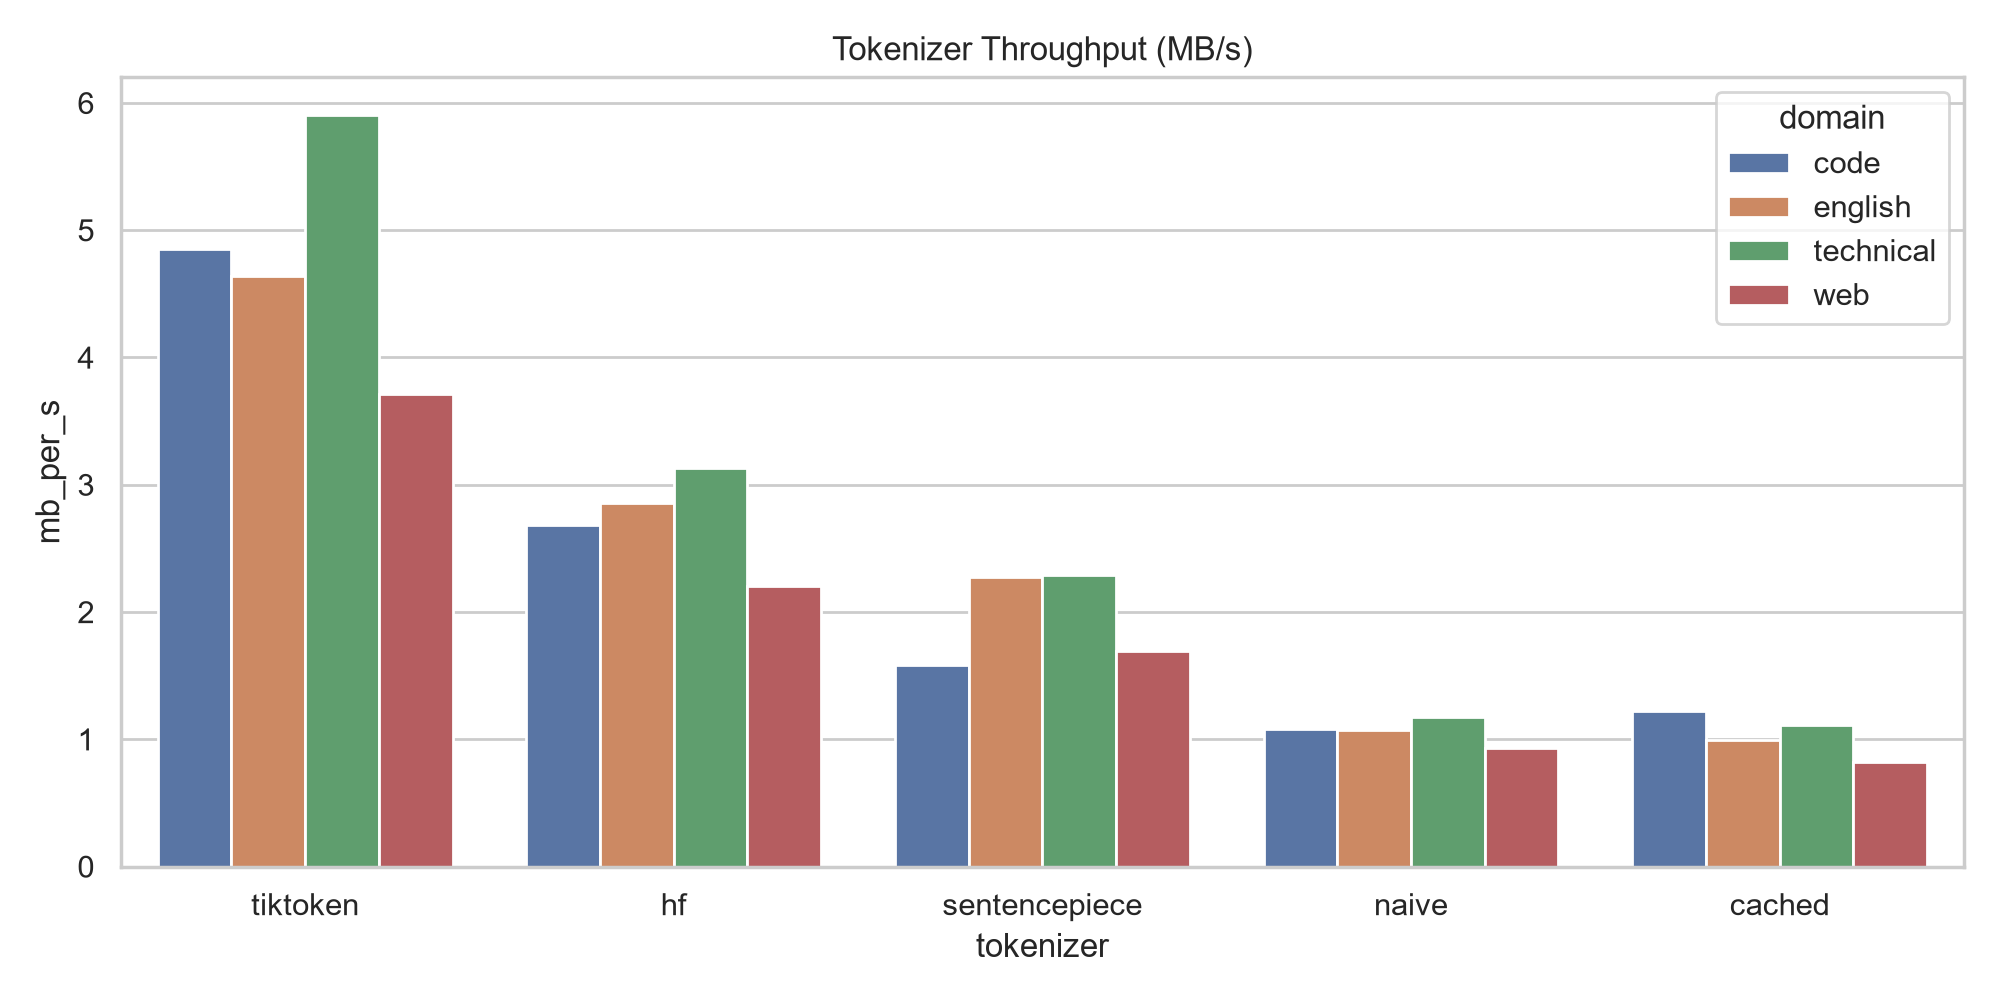
\includegraphics[width=0.85\textwidth]{../results/plots/throughput_mb_s.png}
\caption{Tokenizer throughput comparison in MB/s.}
\label{fig:throughputmb}
\end{figure}

\begin{figure}[H]
\centering
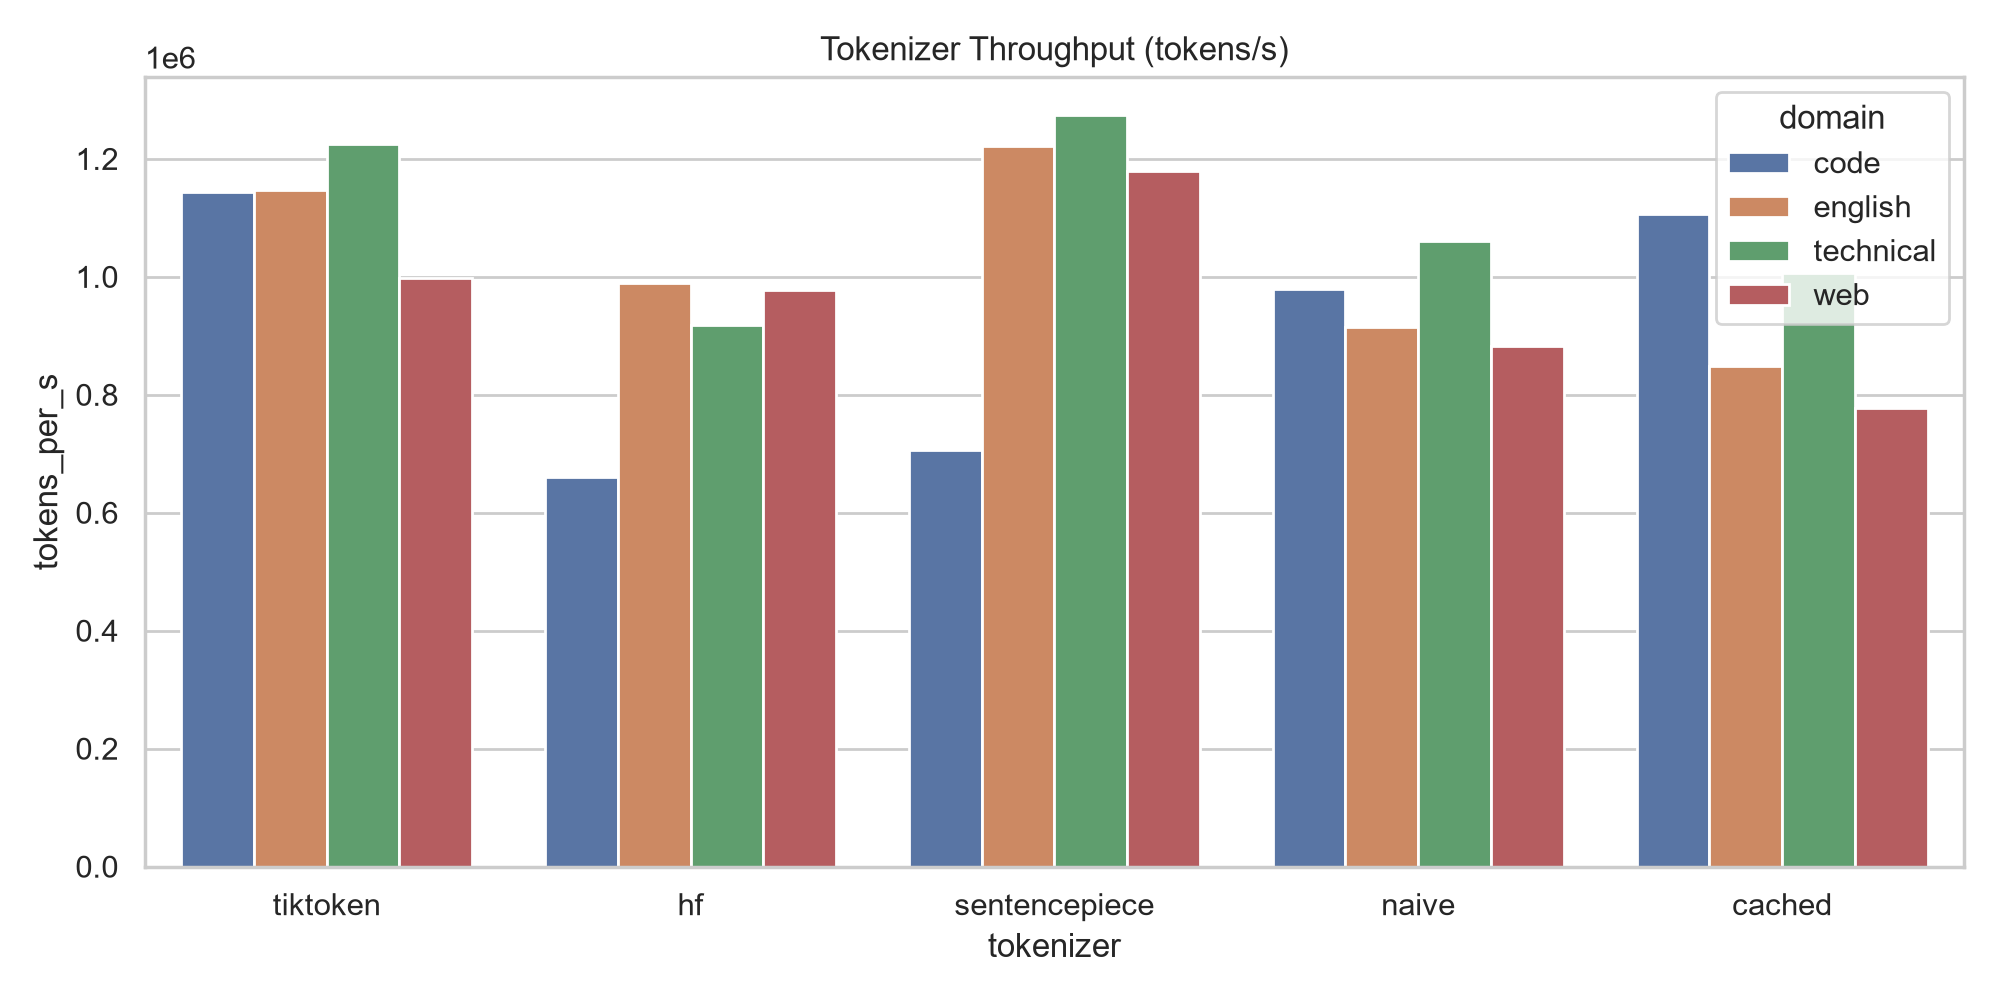
\includegraphics[width=0.85\textwidth]{../results/plots/throughput_tokens_s.png}
\caption{Tokenizer throughput comparison in tokens/s.}
\label{fig:throughputtokens}
\end{figure}

\begin{figure}[H]
\centering
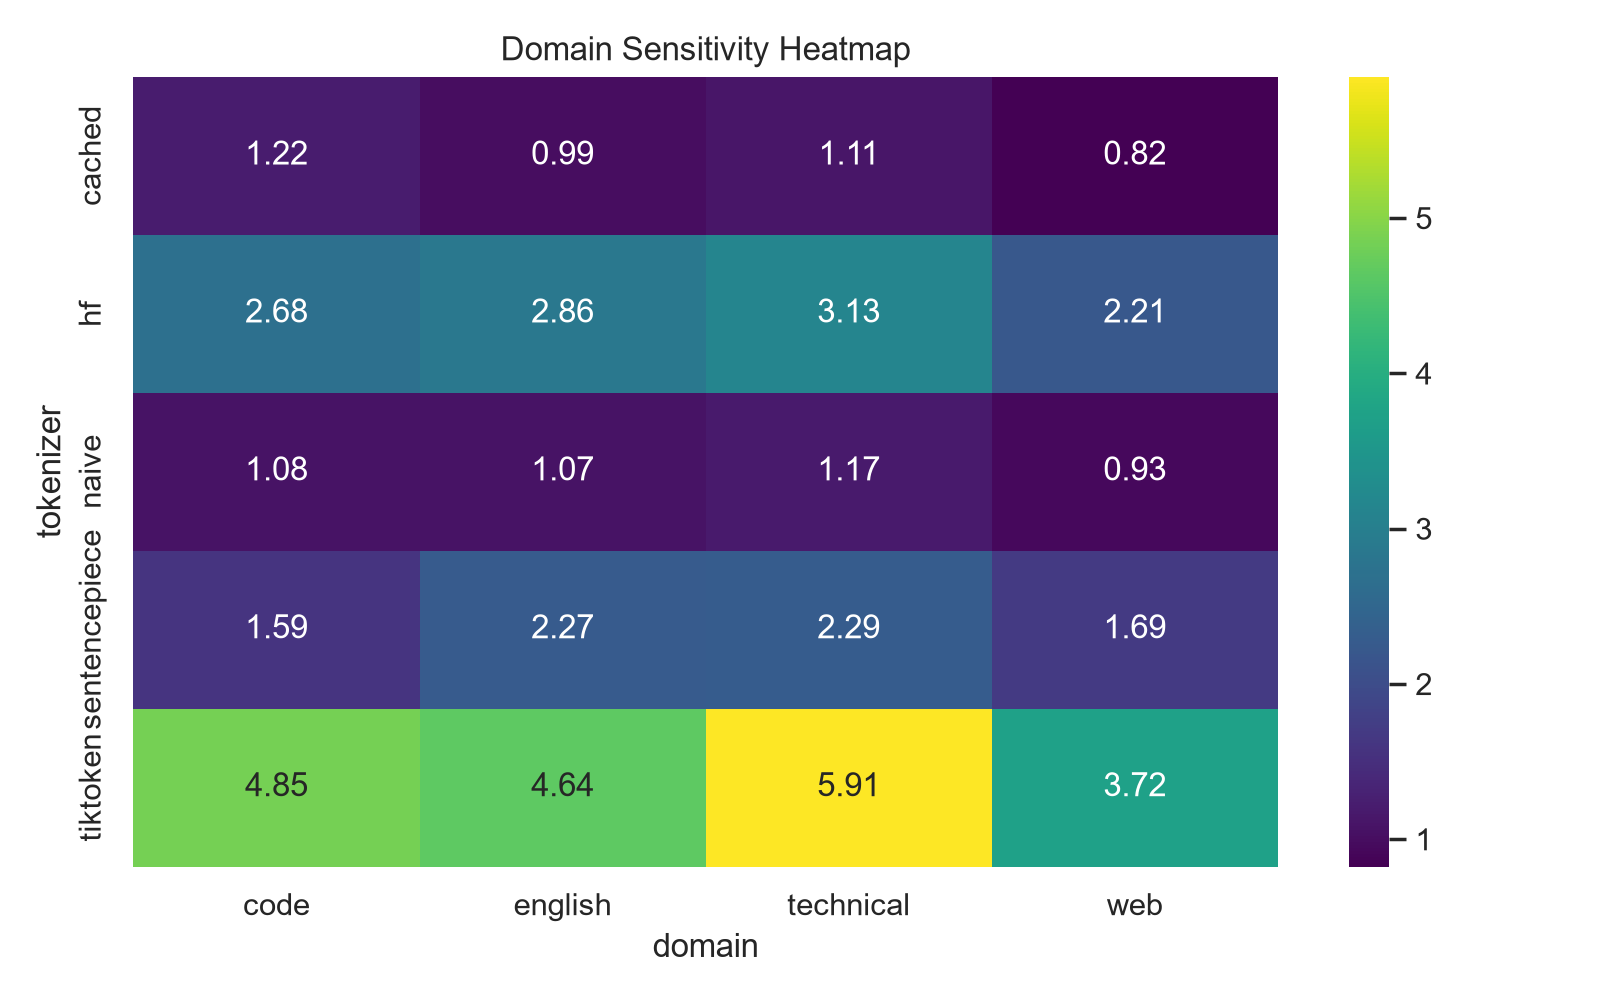
\includegraphics[width=0.85\textwidth]{../results/plots/domain_heatmap.png}
\caption{Domain sensitivity heatmap.}
\label{fig:domainheatmap}
\end{figure}

\begin{figure}[H]
\centering
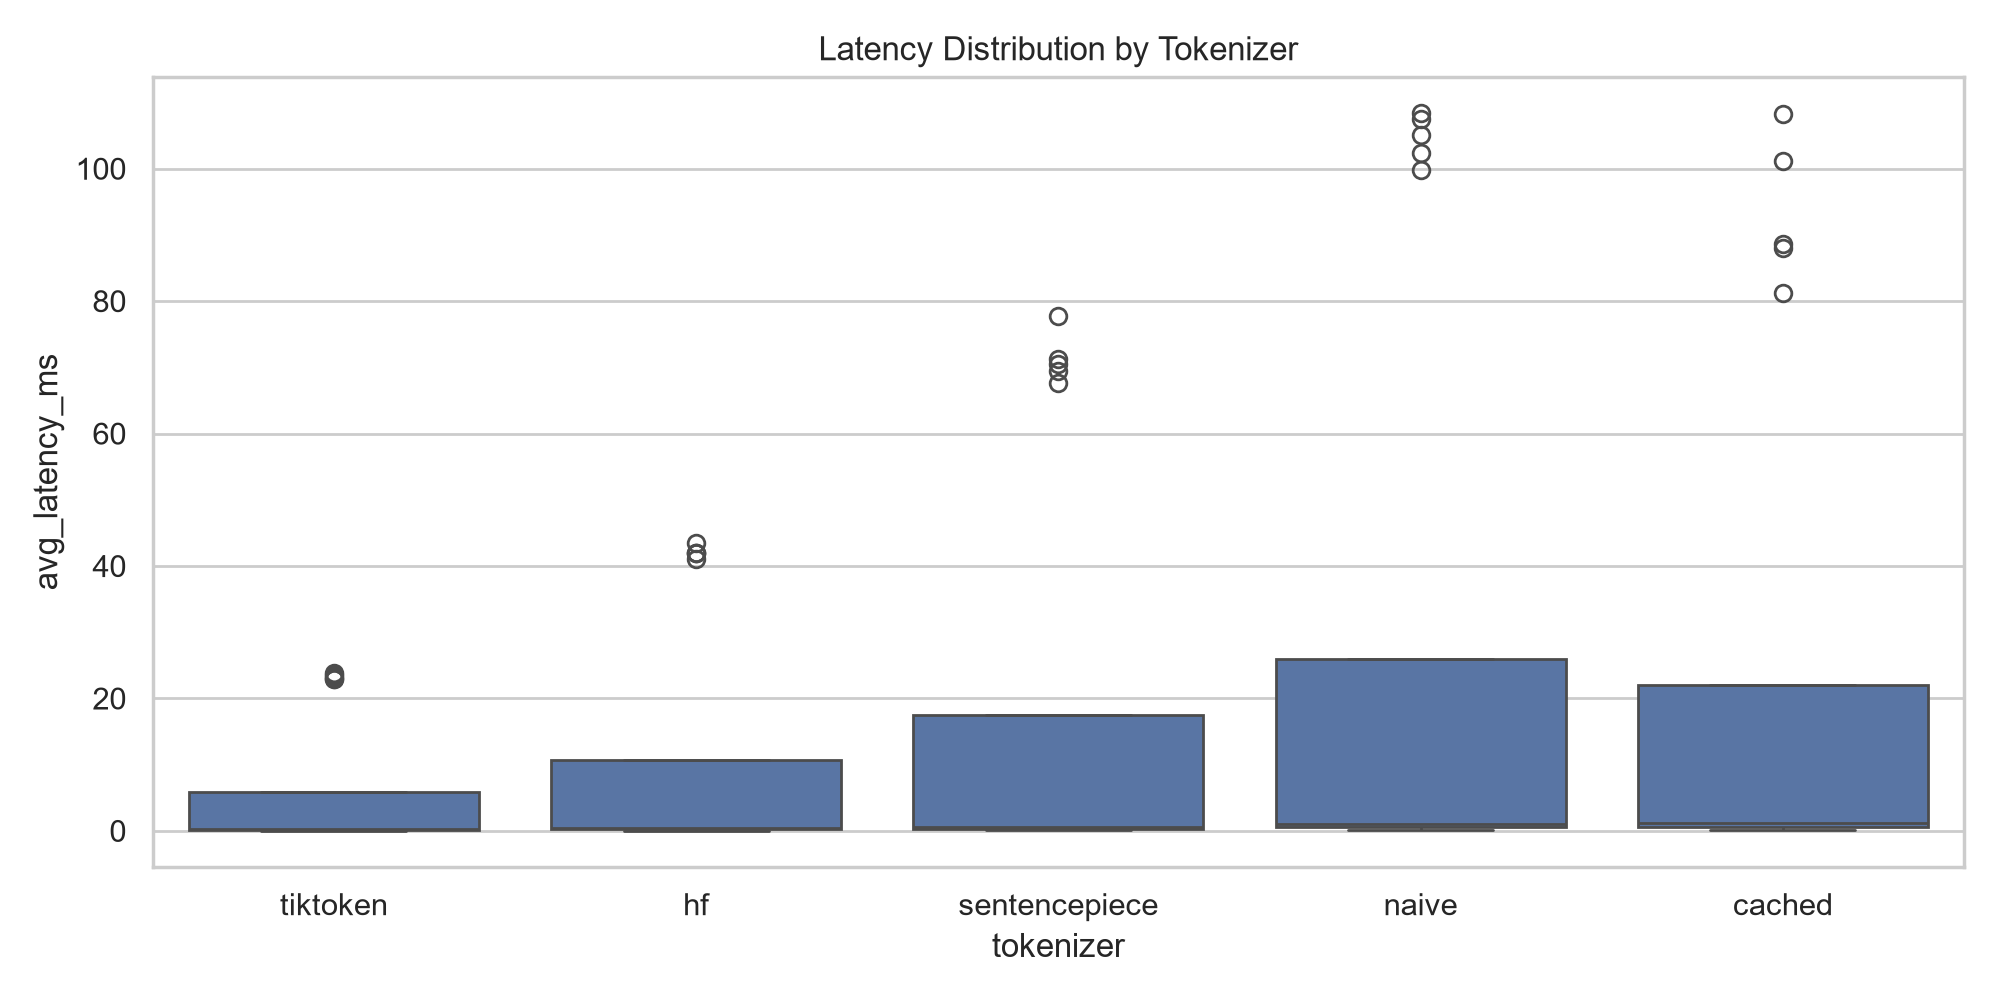
\includegraphics[width=0.85\textwidth]{../results/plots/latency_distribution.png}
\caption{Latency distribution by tokenizer.}
\label{fig:latency}
\end{figure}

\begin{figure}[H]
\centering
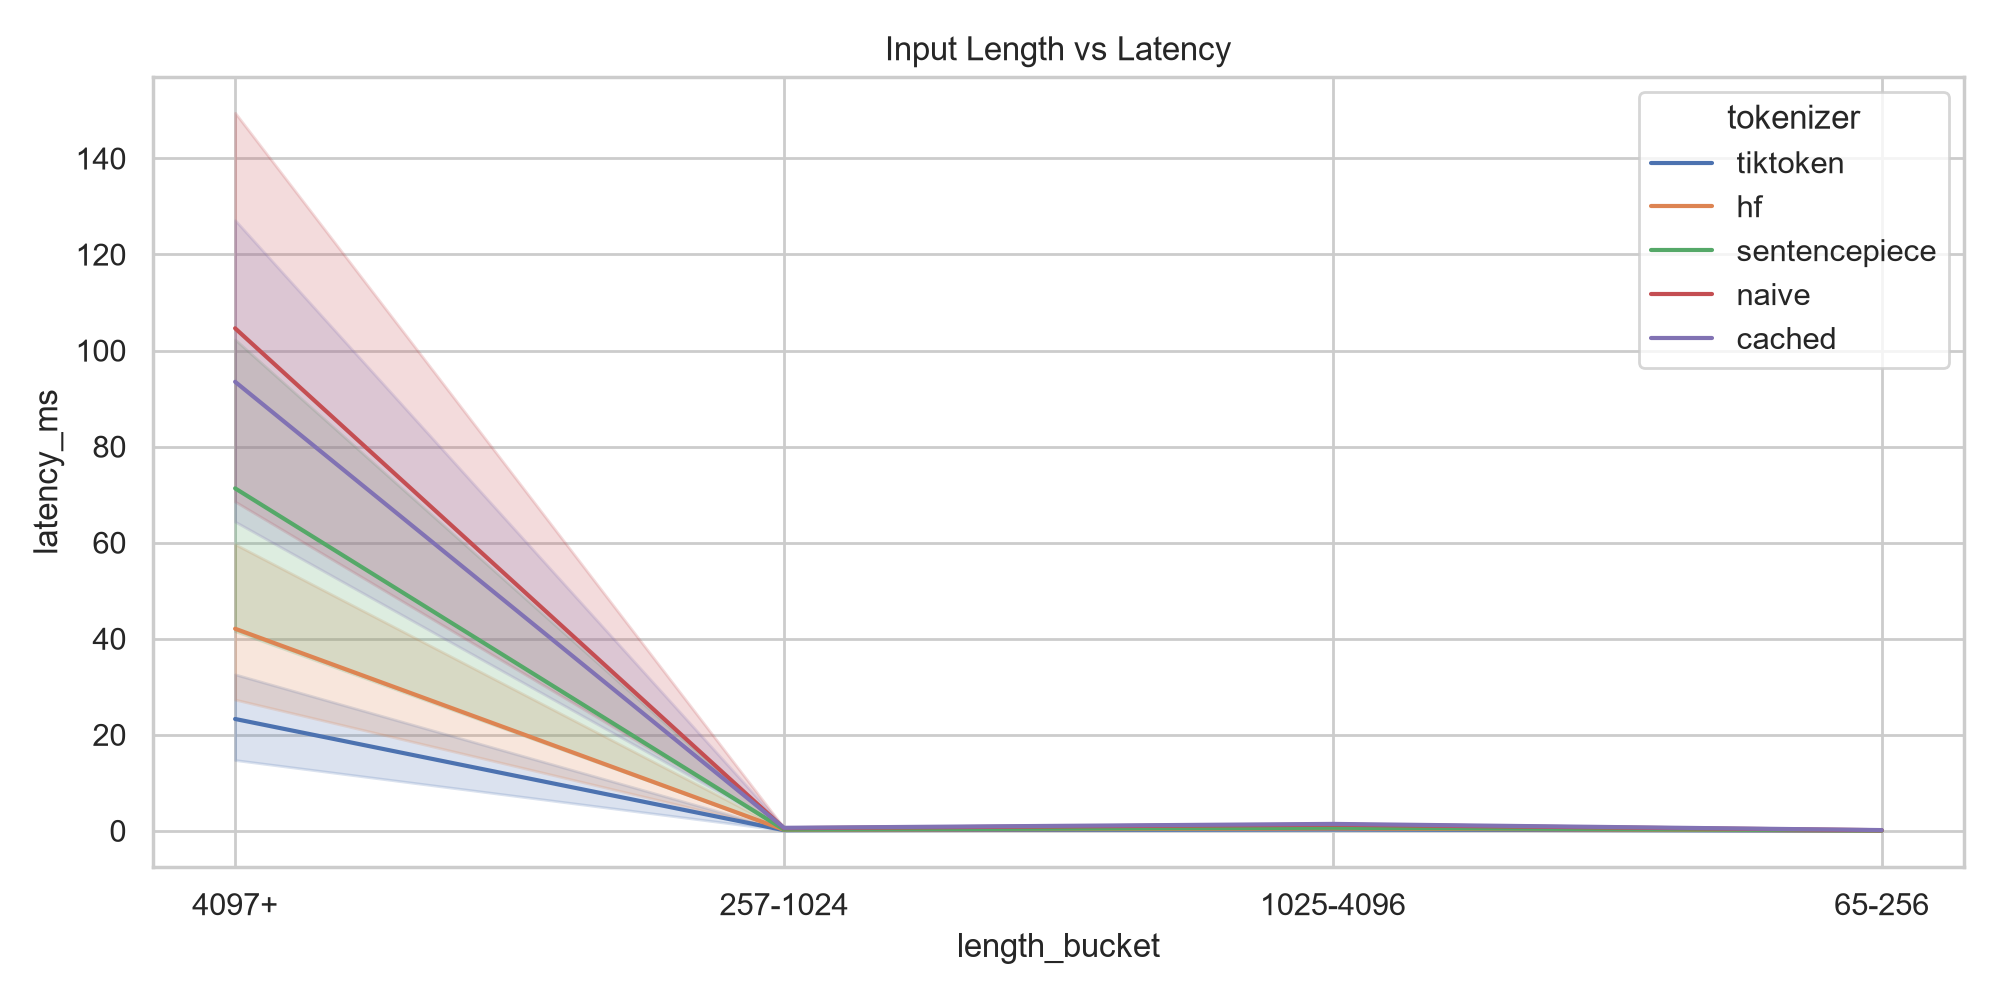
\includegraphics[width=0.85\textwidth]{../results/plots/length_vs_latency.png}
\caption{Input length versus latency.}
\label{fig:lengthlatency}
\end{figure}

\begin{figure}[H]
\centering
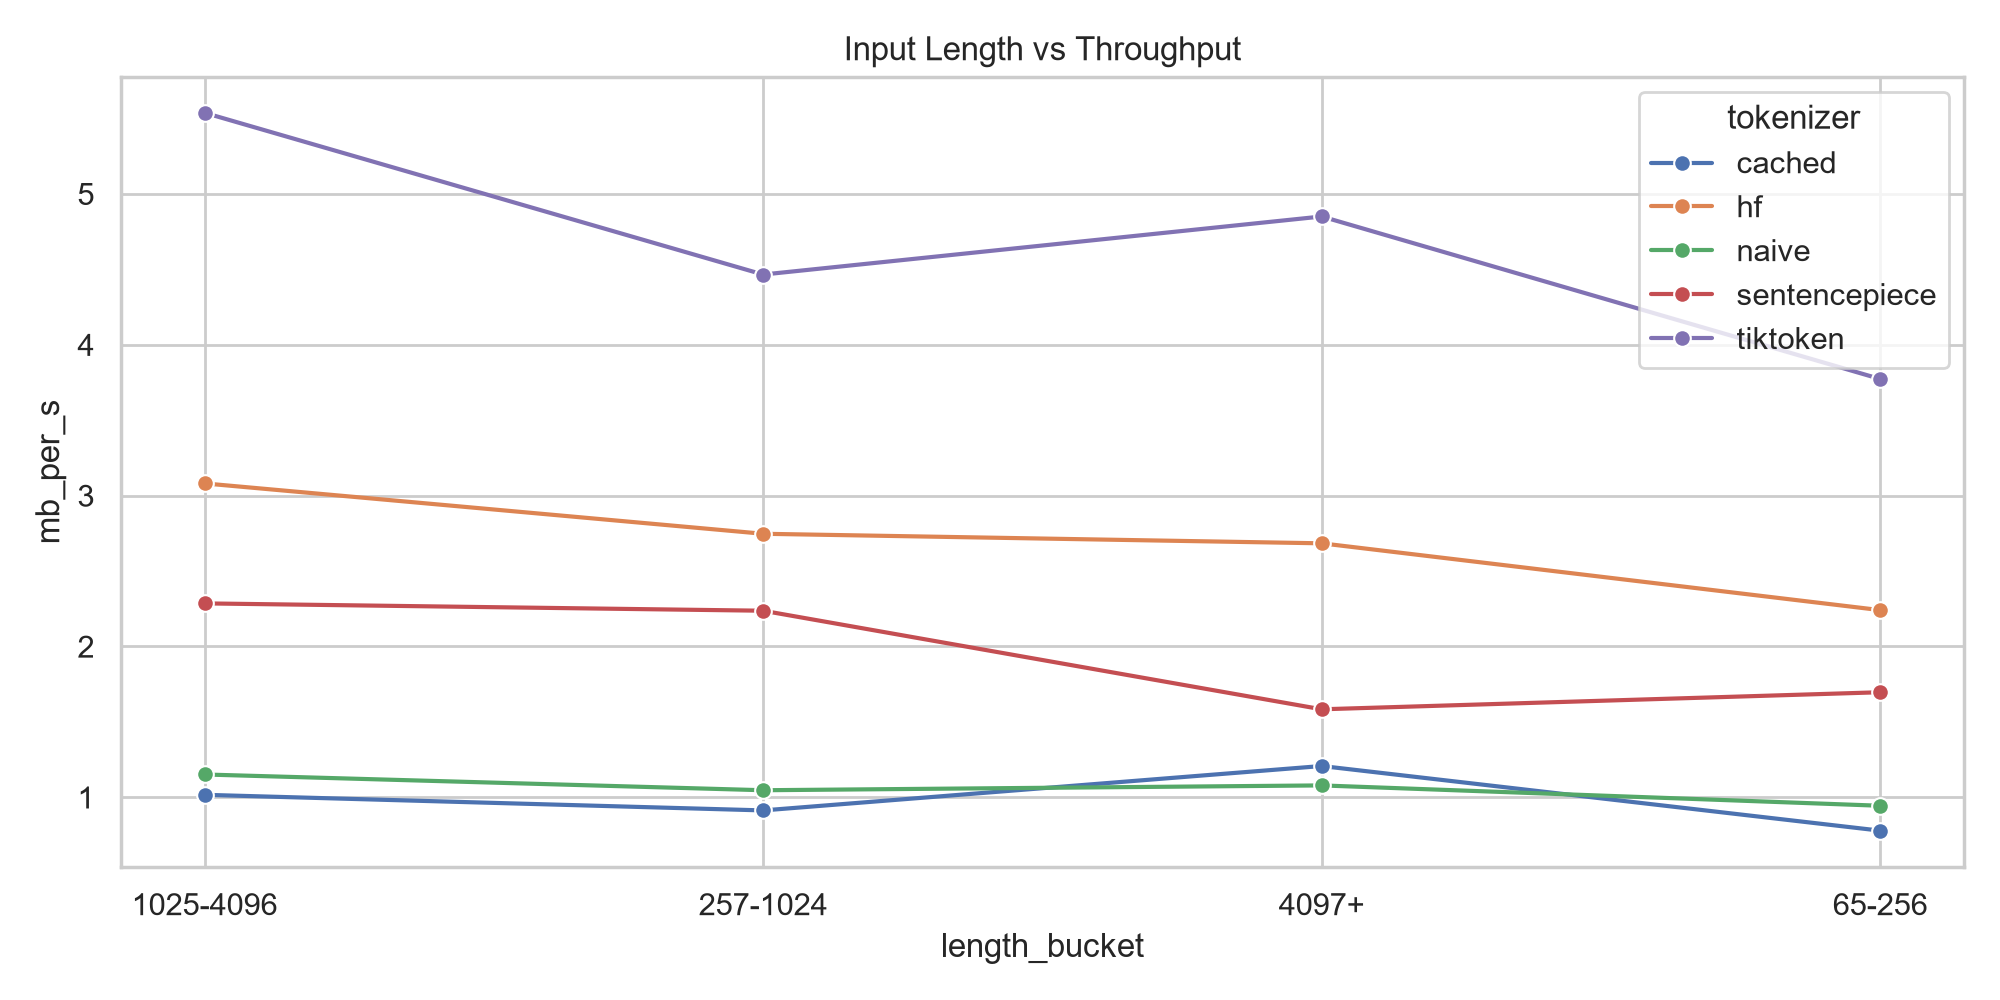
\includegraphics[width=0.85\textwidth]{../results/plots/length_vs_throughput.png}
\caption{Input length versus throughput.}
\label{fig:lengththroughput}
\end{figure}

\begin{figure}[H]
\centering
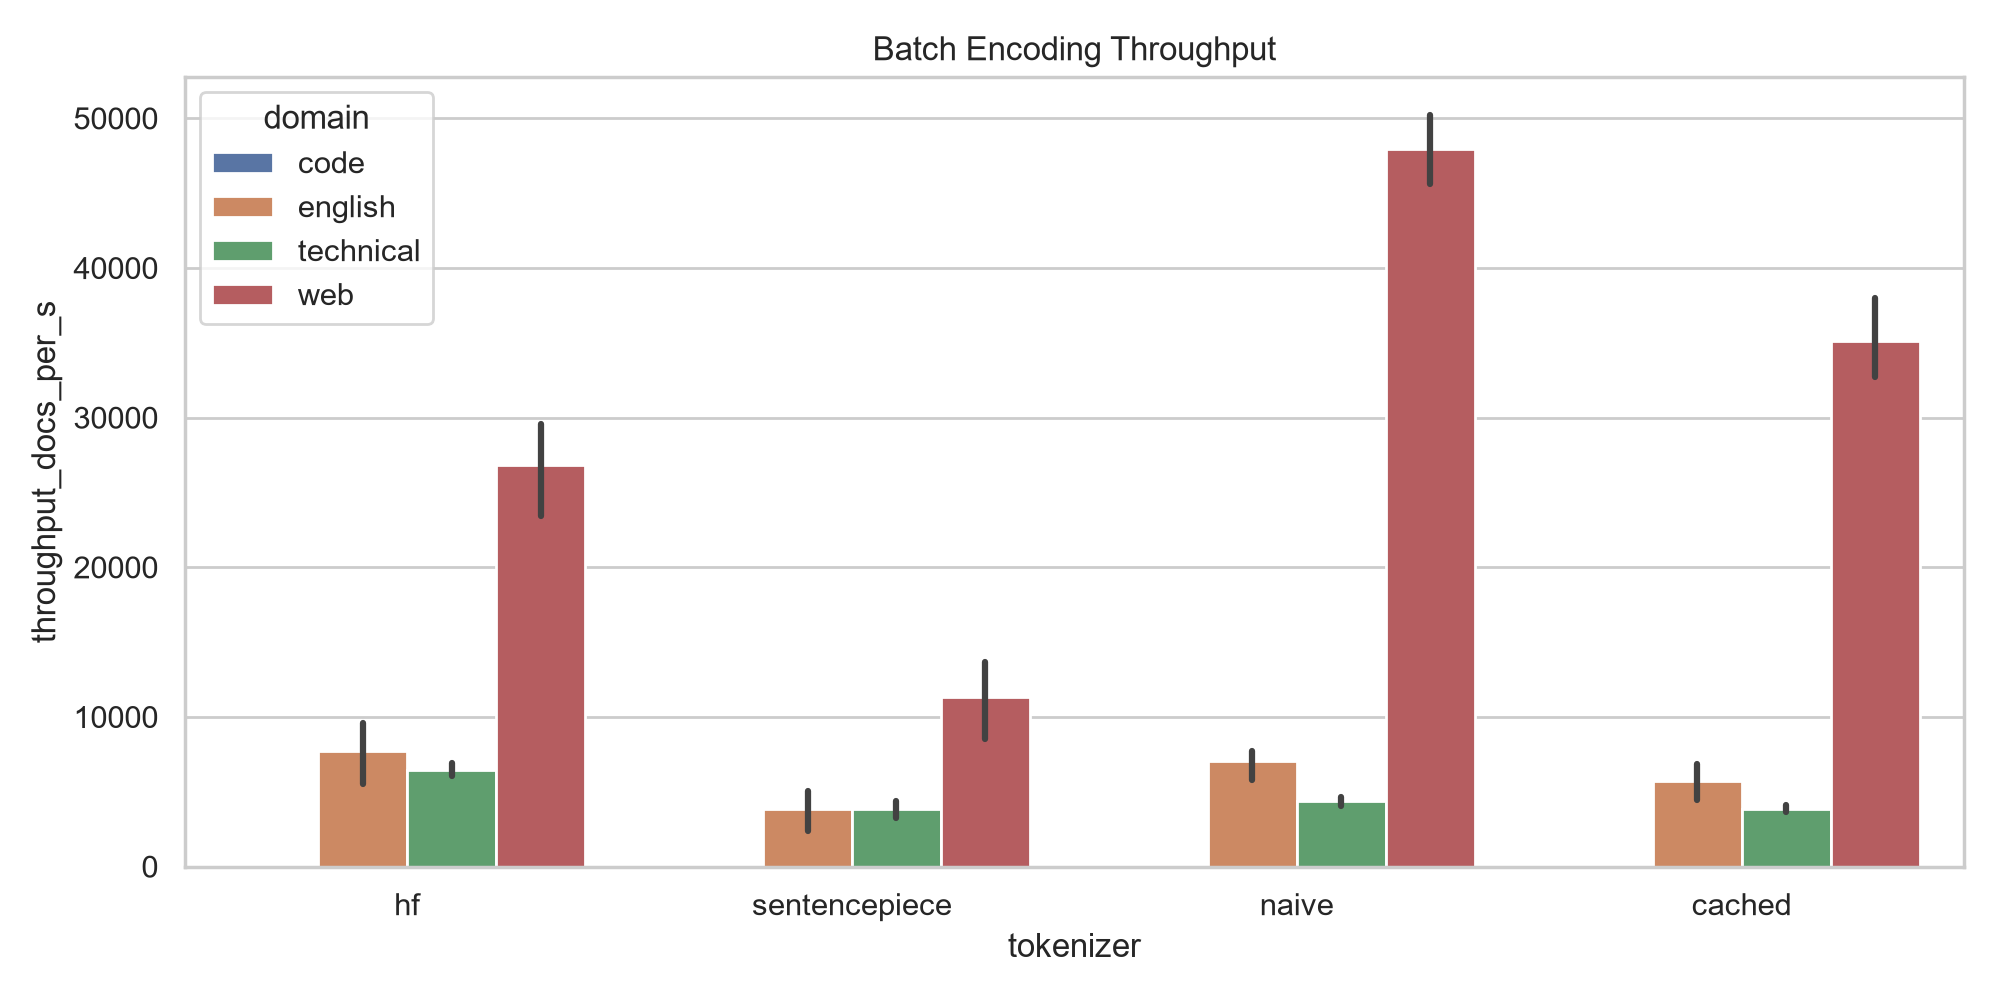
\includegraphics[width=0.85\textwidth]{../results/plots/batch_throughput.png}
\caption{Batch encoding throughput.}
\label{fig:batch}
\end{figure}

\begin{figure}[H]
\centering
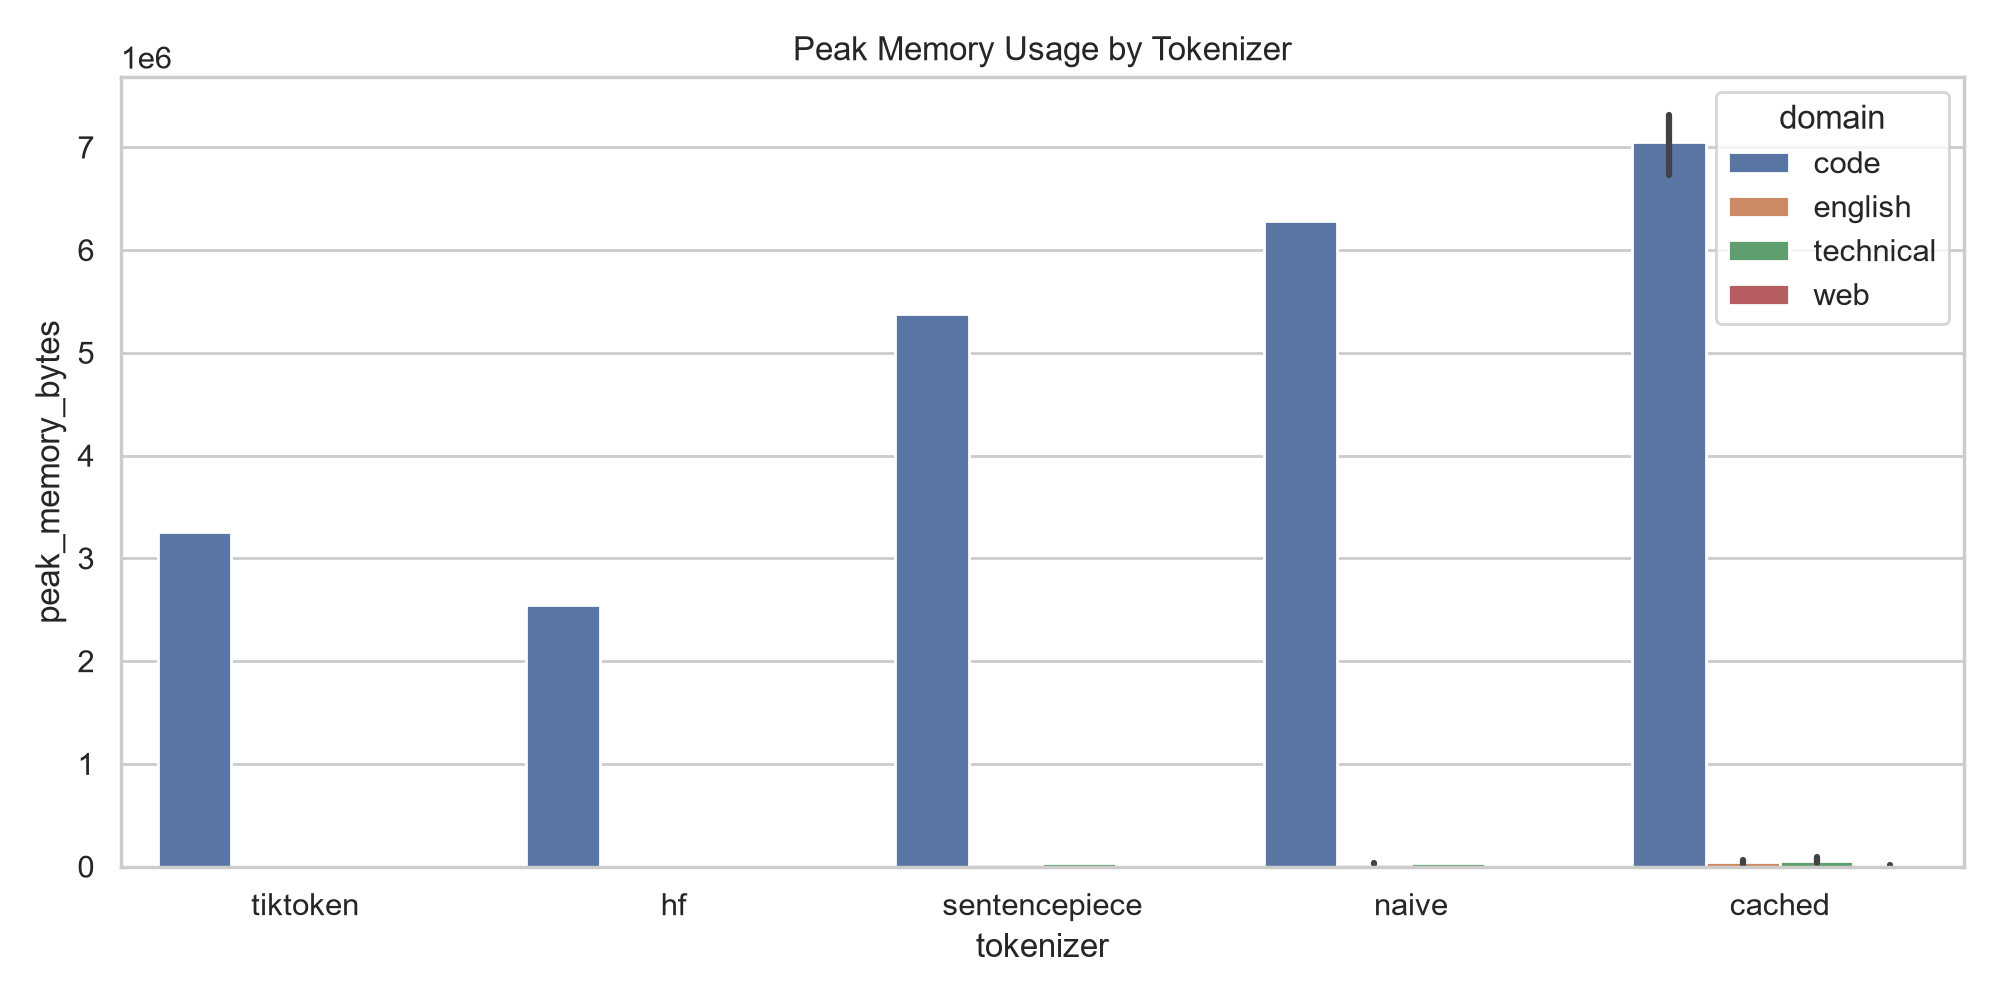
\includegraphics[width=0.85\textwidth]{../results/plots/memory_usage.png}
\caption{Peak memory usage by tokenizer.}
\label{fig:memory}
\end{figure}

\begin{figure}[H]
\centering
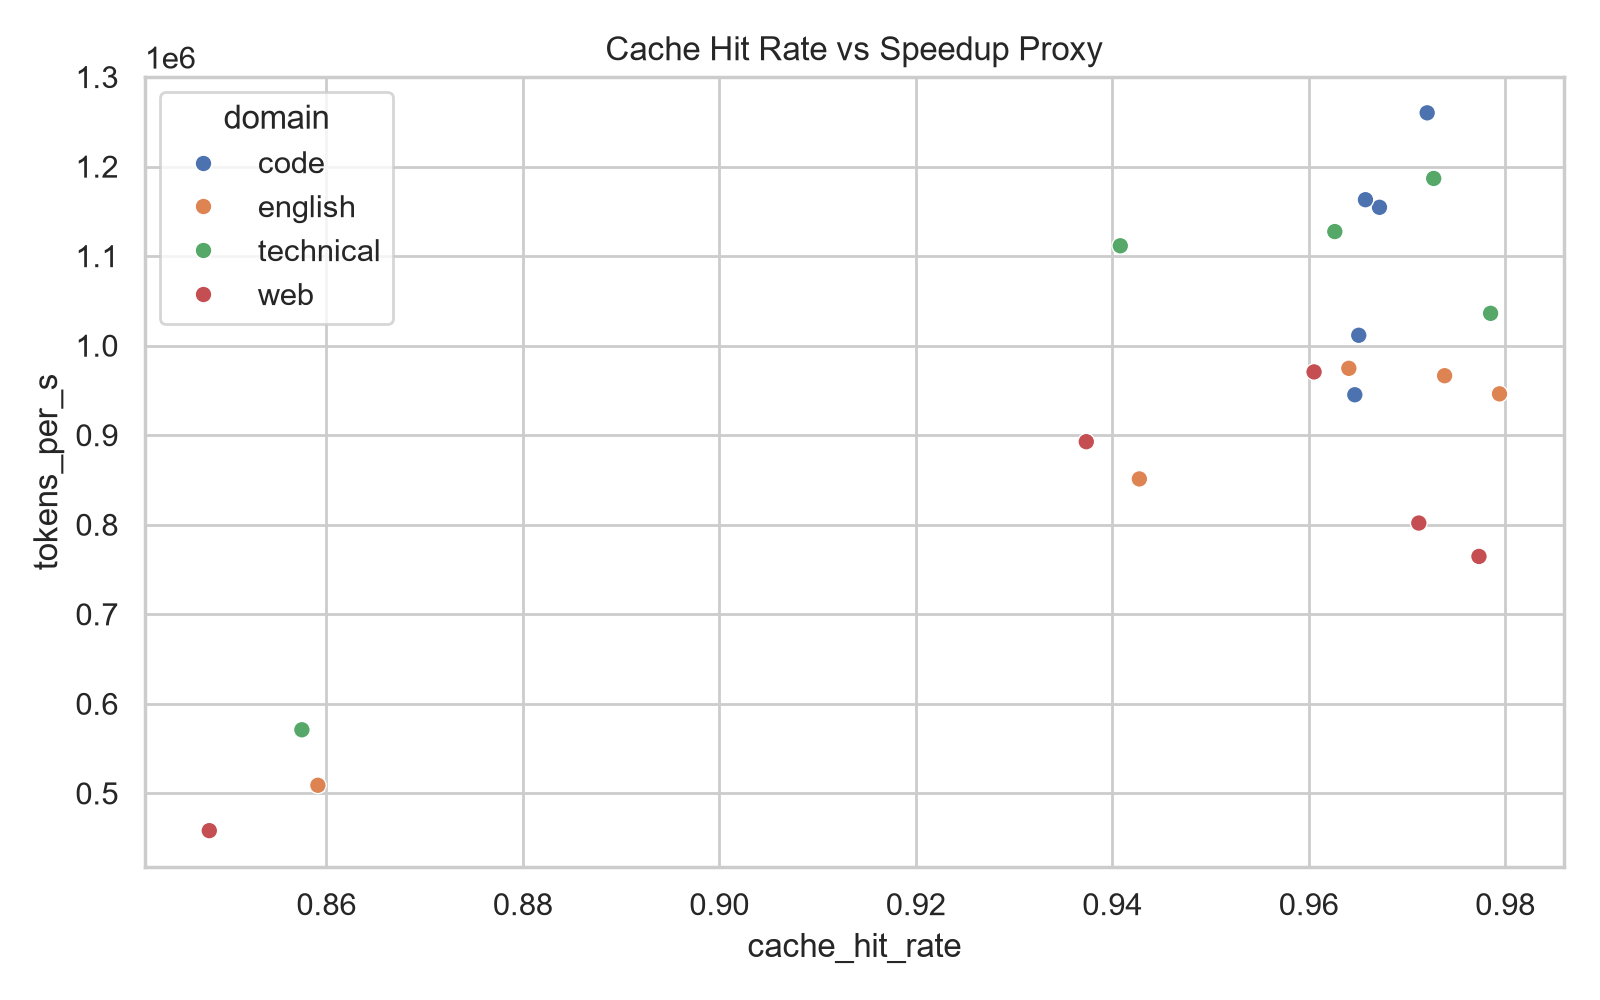
\includegraphics[width=0.85\textwidth]{../results/plots/cache_hit_rate_vs_speedup.png}
\caption{Cache hit rate versus speed proxy for the cached baseline.}
\label{fig:cache}
\end{figure}

\begin{figure}[H]
\centering
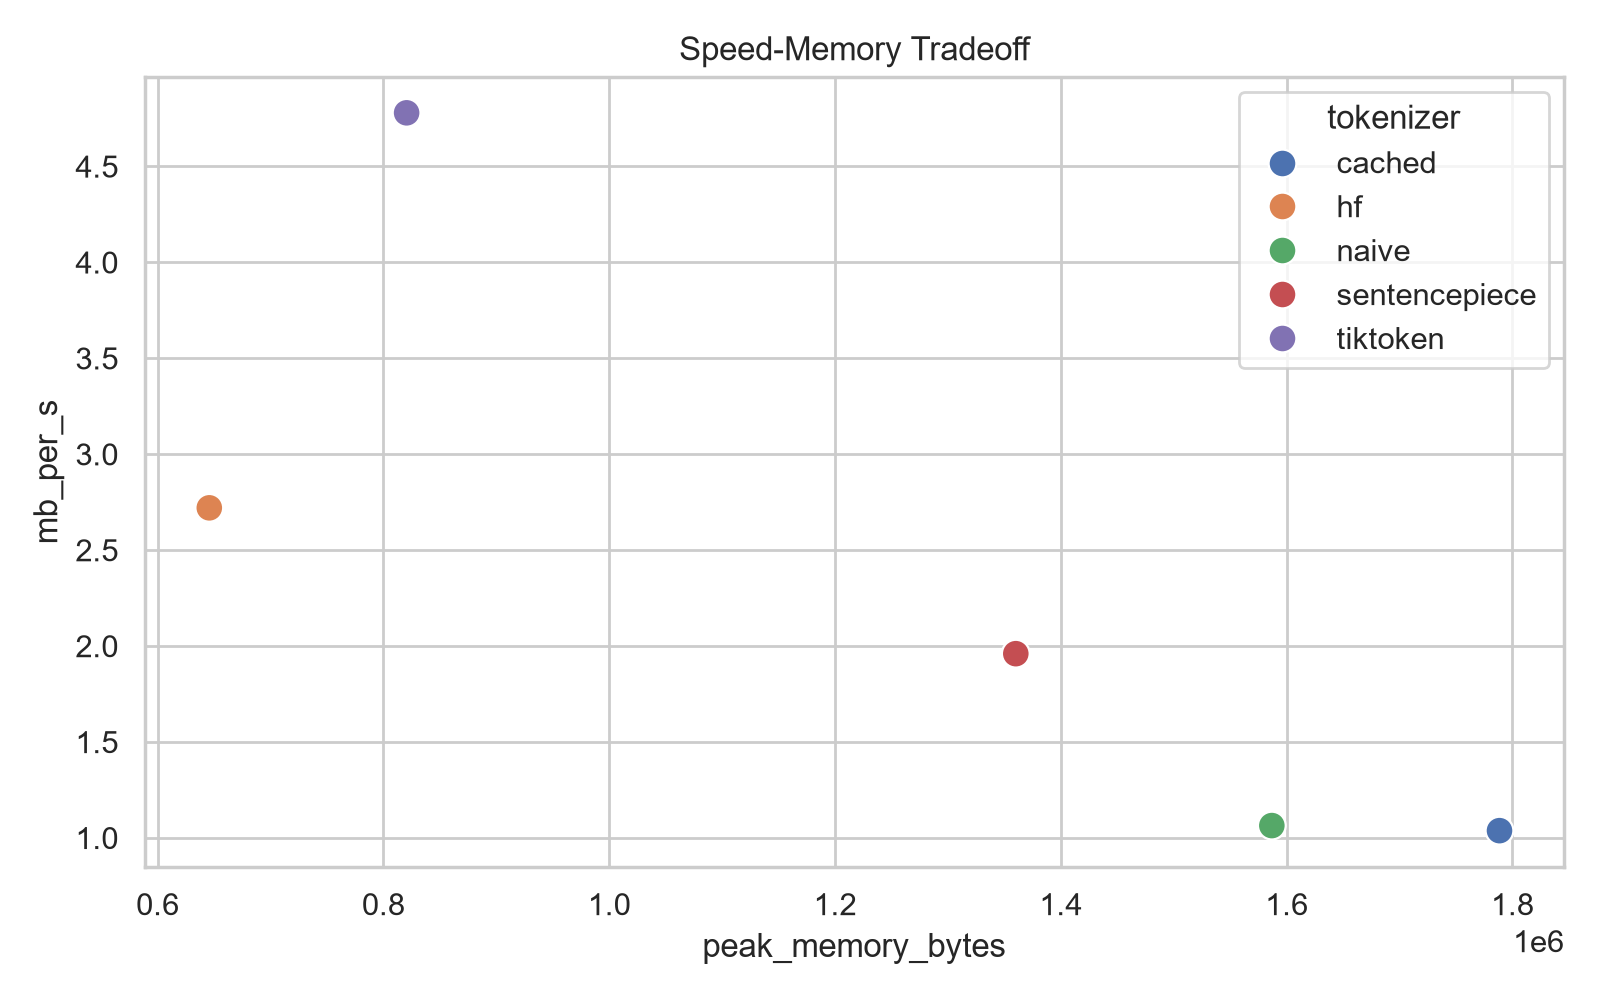
\includegraphics[width=0.85\textwidth]{../results/plots/speed_memory_tradeoff.png}
\caption{Speed-memory tradeoff.}
\label{fig:tradeoff}
\end{figure}

\begin{figure}[H]
\centering
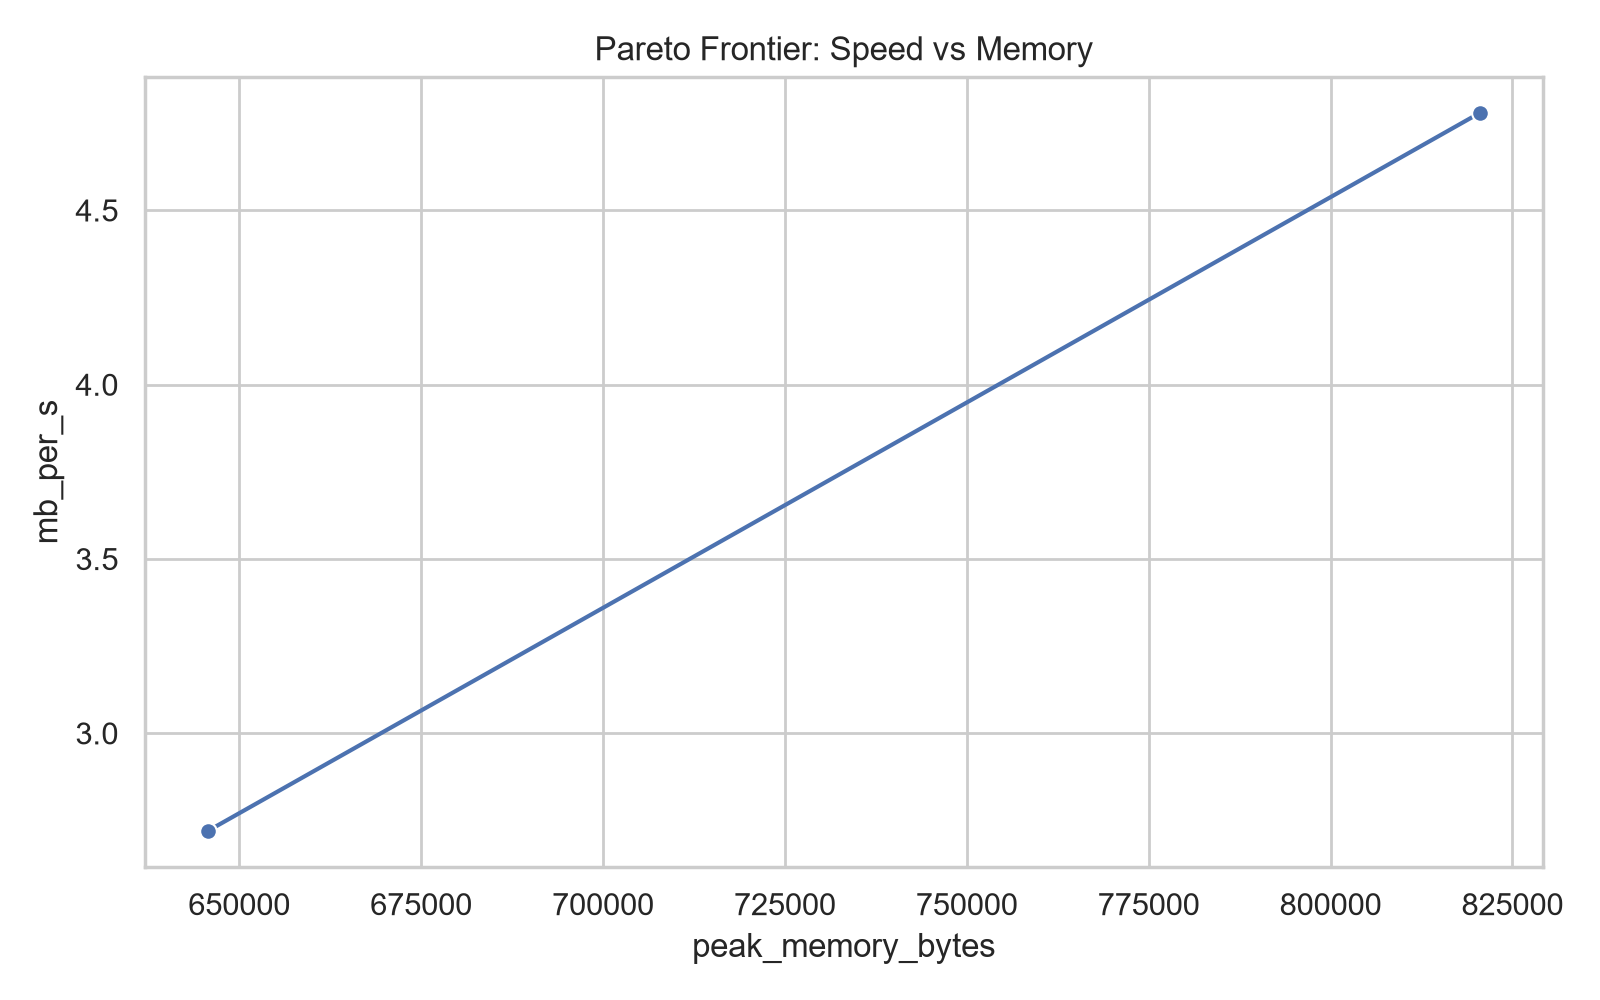
\includegraphics[width=0.85\textwidth]{../results/plots/pareto_frontier.png}
\caption{Pareto frontier of speed versus memory.}
\label{fig:pareto}
\end{figure}

\section{Discussion}
Three results stand out. First, \texttt{tiktoken} was the strongest overall MB/s performer in this run, but SentencePiece remained competitive and surpassed it on the code domain. Second, domain shifts materially changed the ranking, which supports the claim that tokenizer speed cannot be summarized by a single aggregate number without hiding workload structure. Third, repeated-substring caching substantially accelerated the Python baseline, but the associated memory increase and still-nontrivial hit-rate dependence show why optimization must be evaluated as a speed-memory tradeoff rather than as a pure win.

The tokens-per-second ranking differed slightly from the MB/s ranking because different tokenizers emitted different token counts on non-compatible vocabularies. SentencePiece produced the highest average tokens/s even though \texttt{tiktoken} led in MB/s. This is exactly why throughput should be reported in at least both units.

\section{Limitations}
This benchmark run used synthetic but persisted corpora rather than large real datasets from Wikipedia, Git repositories, Reddit, or technical documentation dumps. The custom Python tokenizers are research baselines, not production-quality BPE engines. Exact token-ID compatibility was not tested on a non-reference implementation because the project does not yet include a true \texttt{tiktoken}-compatible optimized tokenizer. As a result, the current findings are strongest on methodology and relative throughput behavior, and weaker on publishable claims about exact accelerated OpenAI-compatible tokenization.

\section{Conclusion}
The current FastBPE run shows that tokenizer performance depends strongly on implementation and domain, and that repeated-substring caching can materially speed up a readable Python baseline. However, the evidence for exact accelerated tokenization remains incomplete until a truly reference-compatible optimized tokenizer is added. The project now has the benchmark, plotting, and reporting infrastructure needed to support that next stage.

\end{document}
